\subsection{Architecture}
\begin{frame}
\frametitle{Xception}
\framesubtitle{Architecture} 

\begin{textblock}{15}(7.67,-0.62)
	\begin{figure}[H]
		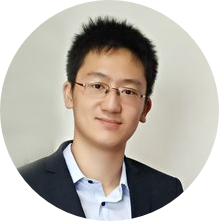
\includegraphics[width=0.1\textwidth]{Images/Team/WeihaoZHOU.png} 
	\end{figure}
\end{textblock}

\begin{textblock}{1}(8.1,1.2)
	\centerline{71 trainable layers ; 22,910,480 parameters}
\end{textblock}

\begin{center}
	
	{\fontsize{8.5}{8}\selectfont
		\begin{tabular}{ccccc}
			\textbf{Layer} & \textbf{Type} & \textbf{Activation function} & \textbf{Output Shape} & \textbf{Param} \\
			input\_1  & (\textcolor{gray}{InputLayer}) & N/A & (299, 299, 3) & \colorbox{yellow}{0} \\         
			block1\_conv1 & (\textcolor{orange}{Conv2D}) & N/A & (149, 149, 32) & 864 \\      
			block1\_conv1\_bn & (\textcolor{red}{Batch Normalization}) & N/A & (149, 149, 32) & 128 \\     
			block1\_conv1\_act & (\textcolor{cyan}{Activation}) & ReLU & (149, 149, 32) & \colorbox{yellow}{0} \\         
			block1\_conv2 & (\textcolor{orange}{Conv2D}) & N/A & (147, 147, 64) & 18,432 \\     
			block1\_conv2\_bn & (\textcolor{red}{Batch Normalization}) & N/A & (147, 147, 64) & 256 \\    
			block1\_conv2\_act & (\textcolor{cyan}{Activation}) & ReLU & (147, 147, 64) & \colorbox{yellow}{0} \\         
			\colorbox{gray}{block2...} & (...) & ... & (147, 147, 128) & ... \\   
			conv2d\_45 & (\textcolor{orange}{Conv2D}) & N/A & (74,74,128) & 8192 \\
			block2\_pool & (\textcolor{blue}{MaxPooling2D}) & N/A & (74,74,128) & \colorbox{yellow}{0} \\
			bn\_45 & (\textcolor{red}{Batch Normalization}) & N/A &(74,74,128) & 512 \\
			add & (\textcolor{violet}{Add}) & N/A & (74,74,128) & \colorbox{yellow}{0} \\
			\colorbox{gray}{block3...} & (...) & ... & (74, 74, 256) & ... \\    
			... & (...) & ... & (...) & ... \\    
			\colorbox{gray}{block14...} & (...) & ... & (10, 10, 1536) & 1,582,080 \\         
			        
			avg\_pool & (\textcolor{blue}{GlobalAveragePooling2D}) & N/A & (, 2048) & \colorbox{yellow}{0} \\          
			predictions & (\textcolor{green}{Dense}) & \textcolor{red}{Softmax} & (, 1000) & 2,049,000   
		\end{tabular}
	}
\end{center}
\end{frame}

\begin{frame}
\frametitle{Xception}
\framesubtitle{Transfer Learning} 

\begin{textblock}{15}(7.67,-0.62)
	\begin{figure}[H]
		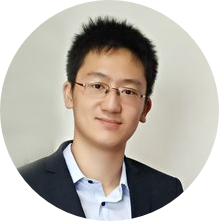
\includegraphics[width=0.1\textwidth]{Images/Team/WeihaoZHOU.png} 
	\end{figure}
\end{textblock}

\begin{center}
	{\fontsize{8.5}{8}\selectfont
		\begin{tabular}{@{\hspace{-0.2cm}}cccc}
			& \textbf{Layer Type} &\textbf{Activation function} & \textbf{Output Shape} \\
			& & \textcolor{white}{phantom} & \\
			\begin{tabular}{c}
				freeze weights\\ learned on ImageNet
			\end{tabular}	
			& $\left\{\begin{tabular}{c}
			(\textcolor{gray}{InputLayer}) \\         
			(\textcolor{orange}{Conv2D}) \\      
			(\textcolor{red}{Batch Normalization}) \\     
			(\textcolor{cyan}{Activation}) \\          
			(...)\\ 
			(...)\\      
			(\textcolor{blue}{GlobalAveragePooling2D}) \\         
			(\textcolor{green}{Dense}) \\ 
			\end{tabular}
			\right.\kern-\nulldelimiterspace$
			& \begin{tabular}{c}
				N/A \\
				N/A \\
				N/A \\
				ReLU \\
				...\\
				...\\
				N/A \\
				ReLU \\
			\end{tabular}
			& \begin{tabular}{c}
				(299, 299, 3) \\
				(149, 149, 32) \\
				(149, 149, 32) \\
				(149, 149, 32) \\
				(...)\\
				(...)\\
				(, 2048) \\
			\end{tabular} \\
			& \hspace{0.2cm} \sout{(\textcolor{green}{Dense})} & \sout{\textcolor{red}{Softmax}} & \sout{(, 1000)} \\
			\only<2>{& \hspace{0.2cm} \textcolor{magenta}{(Dropout)} & N/A & (, 2048) \\} 
			train this layer & \hspace{-1.2cm} $\left\{\begin{tabular}{c}
			\hspace{1.2cm} (\textcolor{green}{Dense})
			\end{tabular} \right.\kern-\nulldelimiterspace$ & \textcolor{red}{Softmax} & \hspace{0.1cm} (, nbClasses)
		\end{tabular}
	}
\end{center}
Trainable params: 6,147
\end{frame}